\section*{Problem statement}
\addcontentsline{toc}{section}{\protect\numberline{}{Problem statement}}

% alignment types
\begin{figure}[t]  %\begin{floatingfigure}[l]{0.5\textwidth}
    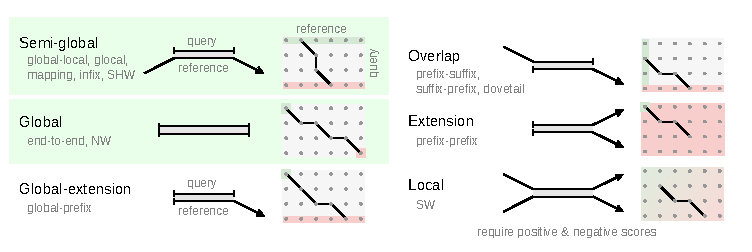
\includegraphics[width=\textwidth]{alignment-types-thesis.pdf}
	\caption[Main alignment types]{Main alignment types. In green are shown the two which are considered in this thesis.}
    \label{fig:alignment-types}
\end{figure}

\paragraph{Sequence alignment}
% problem statements
We consider the problem of pairwise sequence alignment in the context of genomic
data: given two DNA sequences, one can be aligned to the other in multiple
ways~(\cref{fig:alignment-types}). In this thesis we focus on global and
semi-global alignment types only~(marked in green). If both sequences have to be
aligned end to end, we look for a \emph{global alignment} whose minimal number
of edits is known as \emph{edit distance}. If we instead search for an occurance
of a query sequence within a reference sequence, we allow the alignment to start
and end at any reference locations in a \emph{semi-global} alignment.

\paragraph{Objective}
It would have been relatively easy to find alignments if the sequences did not
differ from each other. Nevertheless, the real data may be subject to such
processes as biological evolution and sequencing technologies, which result in
differences between compared sequences. Commonly, the most probable explaination
of these differences is to be reconstructed. If we assume an \emph{error model}
which repeatedly applies a random single-letter edit (substitutions, insertions
and deletions), then the most probable sequence of edits would be one with a
minimal number of edits (possibly weighting different types of edits with
different costs). Throughout this thesis we consider this most widespread
objective -- it provides a tradeoff between expressivity and computability -- it
reasonably estimates the real world sequences while disregarding any memory in
the error model. 

\paragraph{Global alignment}
The simplest type of alignment is to find a sequence of edits that convert one
whole sequence $A$ to another sequence $B$. Note that converting $A$ to $B$
corresponds to the reverse process of converting $B$ to $A$ (e.g. insertions
correspond to deletions). If we ignore the order of applying the edits, the
result can be equivalently represented simpler as an \emph{alignmnet}: each
letter from $A$ has either not been edited (so it corresponded to a matching
letter in $B$), or has been substituted for another letter (so it corresponded
to a mismatching letter in $B$), or has been deleted (which can be represented
as mismatching it with an inserted fictive \emph{gap symbol} in $B$).
Additionally, letters could have been added to $A$ (represented as a gap in $A$
mismatching a letter in $B$). Note that the number of edits is equal to the
number of mismatches in the corresponding alignment. The minimal number of edits
necessary to transform $A$ to $B$ is known as \emph{Levenshtein distance} when
each edit operation is equally costly, and more generally as \emph{edit
distance}, when the edit operations are weighted depending on their type.
Clearly, finding an alignment with a minimal number of edits implies computing
the edit distance. It is unlikely that there exists an algorithm that computes
edit distance in strictly subquadratic time in the worst
case~\cref{backurs2015edit}.

\paragraph{Semi-global alignment}
Semi-global sequence alignment is the alignment of a whole \emph{query} sequence
to a continuous region (subsequence) of a \emph{reference} sequence. This region
is unspecified, so semi-global alignment is a more complex problem than global
alignment. We target semi-global alignment by again minimizing edit distance.
Finding an alignment implies also finding a reference region where the query
aligns, which is known as \emph{mapping}. 

\paragraph{Alignments as shortest paths}

\paragraph{Multiple semi-global alignment (for read mapping)}

\paragraph{Sequence-to-graph alignment (for pangenome references)}
Specifically, a \emph{sequence-to-graph} alignment is a base-to-base
correspondence between a given read and a walk in the graph. As sequencing
errors and biological variation result in inexact read alignments, edit distance
is the most common metric that alignment algorithms optimize in order to find
the most probable read origin in the reference. The shortest path approach
naturally fits more complex references than linear, including even graphs with
cycles.

Formally, we consider the optimal \emph{semi-global alignment} problem,
the task of finding an optimal base-to-base correspondence between a query
sequence and a (possibly cyclic) walk in the graph. Related alignment problems
have already been formulated as graph shortest path
problems~\cite{jain_complexity_2019}.
 (also called approximate/fuzzy string search outside computational
biology).
We note that in contrast to linear references, reference graphs capture genomic
variation and therefore enable more accurate semi-global
alignments~\citep{garrison_variation_2018}.